\documentclass{article}

\usepackage[]{xrcise}

\subject{Machine Learning}
\semester{Summer 2025}
\author{Leopold Lemmermann}

\begin{document}
\createtitle

\sheet[2024]{First Exam}

\begin{exercise}{Multiple Choice}
  \begin{enumerate}
    \item Which of the following functions is convex?
      \begin{itemize}
        \item $f(x) = ||x||_1 - 1$, $x \in \mathbb{R}^d$
        \item $f(x) = e^x$, $x \in \mathbb{R}$
        \item $f(x) = \max(0, |x|)$, $x \in \mathbb{R}$
      \end{itemize}
    \item Which are the effects of ensemble learning when applied to Decision Trees using Random Forests?
      \begin{itemize}
        \item Reduces bias, increases variance
        \item Reduces variance, increases bias
        \item Can be used to avoid overfitting
        \item Can be used to avoid underfitting
      \end{itemize}
    \item Which statements are true about the k-NN algorithm?
      \begin{itemize}
        \item Increasing $k$ increases model variance
        \item Increasing $k$ increases model bias
        \item You can use it for regression
        \item You can also use the L1-norm as a distance metric
      \end{itemize}
    \item Which statements are true about k-means?
      \begin{itemize}
        \item It is sensitive to noisy data or many outliers
        \item It always converges
        \item It always finds an optimal solution
      \end{itemize}
    \item What is correct with respect to QDA?
      \begin{itemize}
        \item It's a generative model.
        \item It can be used for regression.
        \item It assumes that each individual data point follows a certain Gaussian distribution and that all of these distributions have the same covariance matrix.
      \end{itemize}
    \item Which statements are true about Naive Bayes?
      \begin{itemize}
        \item You can classify more than one class with it.
        \item Together with Laplacian smoothing it can be used for regression.
      \end{itemize}
    \item Which statements are true about PCA?
      \begin{itemize}
        \item PCA is a clustering algorithm.
        \item In PCA, the variance of the projected data points is maximized.
        \item PCA uses linear combinations of the input features for the transformation.
      \end{itemize}
  \end{enumerate}

  \begin{solution}
    \begin{enumerate}
      \item \textbf{Convex functions:} $f(x) = ||x||_1 - 1$ is convex, $f(x) = e^x$ is convex, $f(x) = \max(0, |x|)$ is convex.
      \item \textbf{Ensemble learning effects:} Reduces variance, increases bias; can be used to avoid overfitting.
      \item \textbf{KNN statements:} Increasing $k$ increases model bias; you can use it for regression; you can also use the L1-norm as a distance metric.
      \item \textbf{k-means statements:} It is sensitive to noisy data or many outliers; it always converges.
      \item \textbf{QDA statements:} It's a generative model; it can be used for regression.
      \item \textbf{Naive Bayes statements:} You can classify more than one class with it.
      \item \textbf{PCA statements:} In PCA, the variance of the projected data points is maximized; PCA uses linear combinations of the input features for the transformation.
    \end{enumerate}
  \end{solution}
\end{exercise}

\begin{exercise}{SVMs}
  \begin{enumerate}
    \item What is the base assumption (inductive bias) about your data if you use an SVM?
    \item How do Hard-margin SVMs differ from Soft-margin SVMs?
    \item Given the plot, draw the decision boundaries for a hard margin and a soft margin SVM and mark them properly.
      \begin{figure}
        \centering
        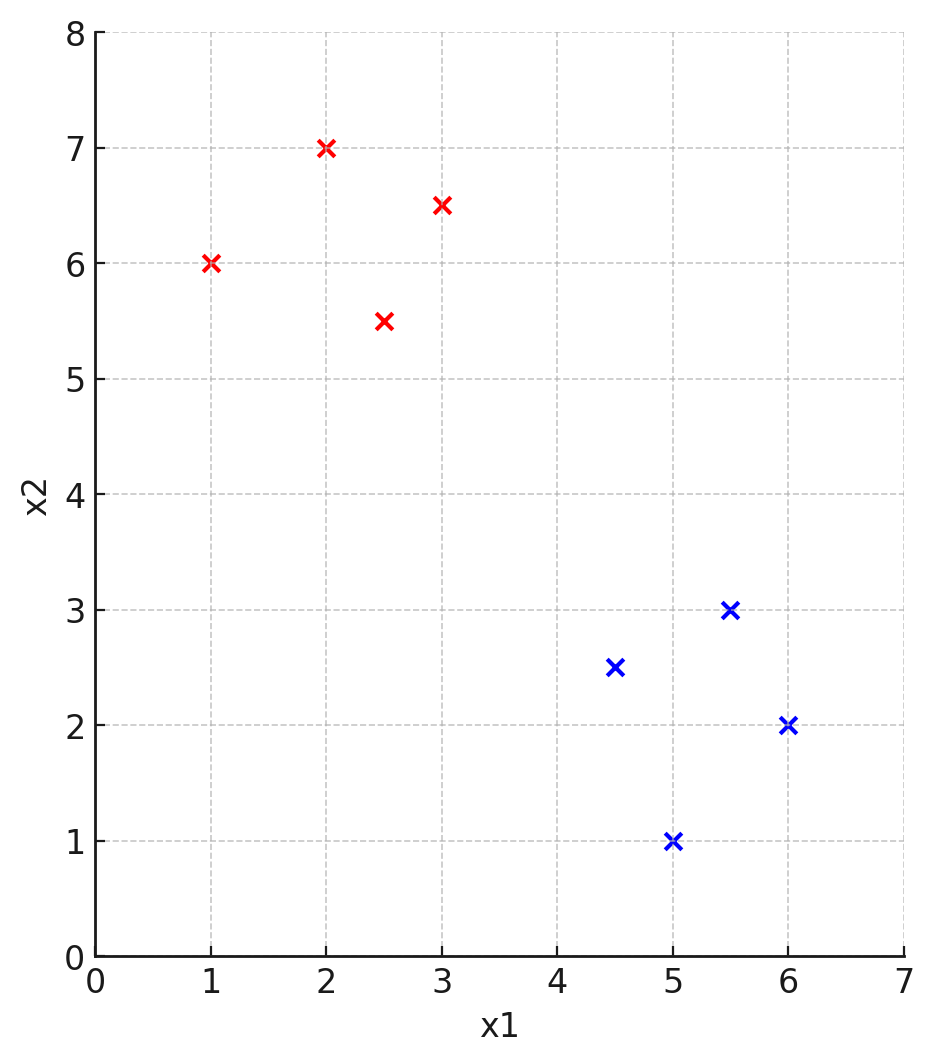
\includegraphics[width=0.5\textwidth]{res/svm_decision_boundary.png}
        \caption{Decision boundaries for SVMs}
        \label{fig:svm_decision_boundary}
      \end{figure}
  \end{enumerate}

  \begin{solution}
    \begin{enumerate}
      \item The base assumption is that the data is linearly separable.
      \item Hard-margin SVMs require perfect separation of classes, while soft-margin SVMs allow for some misclassification to handle noise.
      \item The decision boundary for a hard-margin SVM is a straight line that separates the classes with the maximum margin, while the soft-margin SVM allows for some points to be within the margin or misclassified, resulting in a more flexible boundary.
    \end{enumerate}
  \end{solution}
\end{exercise}

\begin{exercise}{Covariance and Kernel Matrix}
  You are given the three data points (0,1), (1,-2), (-1,1).
  \begin{enumerate}
    \item Compute the covariance matrix and the kernel matrix (aka Gram matrix).
    \item In general, what are the dimensions of the Covariance Matrix and the Kernel Matrix for an input Matrix of $n \times d$?
  \end{enumerate}

  \begin{solution}
    The covariance matrix is:
    \[
      \text{Cov}(X) = \begin{pmatrix}
        0 & 1 \\
        1 & -2 \\
        -1 & 1
      \end{pmatrix}
    \]
    The kernel matrix is:
    \[
      K = \begin{pmatrix}
        1 & 0 & -1 \\
        0 & 4 & -2 \\
        -1 & -2 & 1
      \end{pmatrix}
    \]
    The dimensions of the Covariance Matrix are $d \times d$ and for the Kernel Matrix are $n \times n$.
  \end{solution}
\end{exercise}

\begin{exercise}{Isomap}
  \begin{enumerate}
    \item What is the objective of isomap and how does it differ from PCA? (2 sentences)
    \item Describe the steps of the isomap algorithm (3 sentences).
    \item Is isomap a supervised or an unsupervised ML algorithm and why? (1 sentence)
  \end{enumerate}

  \begin{solution}
    \begin{enumerate}
      \item The objective of isomap is to preserve the geodesic distances between points in a manifold, while PCA focuses on maximizing variance. Isomap captures nonlinear structures, whereas PCA assumes linear relationships.
      \item The steps of the isomap algorithm include: 1) Compute pairwise geodesic distances between points using Dijkstra's algorithm, 2) Construct a low-dimensional embedding by applying classical MDS to the distance matrix, and 3) Project the data into the lower-dimensional space.
      \item Isomap is an unsupervised learning algorithm because it does not rely on labeled data for its computations.
    \end{enumerate}
  \end{solution}
\end{exercise}

\begin{exercise}{Ridge Regression Solver}
  You have the problem: 
    \[ \min_{w} \sum_{i=1}^{n} \left( \left(x^{(i)}\right)^T w - y^{(i)} \right)^2 + \lambda \sum_{j=1}^{m} \alpha_j w_j^2 \]
  With scikit-learn only, the solver for ridge regression (i.e., $\|Xw - y\|_2^2 + \alpha\|w\|_2^2$) is provided. How can you change the problem and still use the ridge regression solver implemented in scikit-learn? Provide a mathematical derivation of your solution.

  \begin{solution}
    The problem can be transformed by introducing a new variable $w' = \sqrt{\lambda} w$. The objective becomes:
    \[
      \min_{w'} \sum_{i=1}^{n} \left( \left(x^{(i)}\right)^T \frac{1}{\sqrt{\lambda}} w' - y^{(i)} \right)^2 + \sum_{j=1}^{m} \left(w'_j\right)^2
    \]
    This allows us to use the ridge regression solver in scikit-learn, as it now matches the form of the ridge regression problem.
  \end{solution}
\end{exercise}

\begin{exercise}{Matrix}
  You are given a rating matrix and since you know that there are a lot of outliers in the data, you choose the L1 norm instead of the L2 norm. Come up with an algorithm that is similar to ALS that solves this problem (pseudocode preferred) and also derive the mathematical reason for your solution.
    \[ \min_{U, V} \|R - UV^T\|_{1,\Omega} \]
    \[ \|A\|_{1,\Omega} = \sum_{i,j} |a_{i,j}| \]

  \begin{solution}
    The algorithm can be derived as follows:
    \begin{enumerate}
      \item Initialize $U$ and $V$ randomly.
      \item For each iteration:
        \begin{itemize}
          \item Fix $U$ and update $V$ by solving:
            \[
              V = \arg\min_{V} \sum_{i,j \in \Omega} |R_{i,j} - U_i V_j^T| + \lambda \|V\|_1
            \]
          \item Fix $V$ and update $U$ similarly.
        \end{itemize}
      \item Repeat until convergence.
    \end{enumerate}
    The mathematical reason is that the L1 norm leads to a sparse solution, which is beneficial in the presence of outliers. The optimization alternates between updating $U$ and $V$, similar to ALS, but uses L1 regularization to handle the outliers effectively.
  \end{solution}
\end{exercise}

\begin{exercise}{Python}
  You are given the following Python code:

  \medskip
  \texttt{def foo(X, y, alpha):}\\
  \texttt{\ \ m,n = X.shape}\\
  \texttt{\ \ th = np.random.randn(1,n)}\\
  \texttt{\ \ for \_ in range(1000):}\\
  \texttt{\ \ \ \ u = 2/m * X.T.dot(X.dot(th) - y) + 2 * alpha * th}\\
  \texttt{\ \ \ \ th -= 1e-3 * u}\\
  \texttt{\ \ return th}

  What problem is being solved, and what do the variables represent?

  \begin{solution}
    This code implements a gradient descent algorithm for ridge regression.  
    - $X$: design matrix of features.
    - $y$: target vector.
    - $\alpha$: regularization parameter.
    - $th$: parameter vector being learned.
    The update step includes the gradient of squared error and an L2 penalty term.
  \end{solution}
\end{exercise}

\begin{exercise}{Regularization}
  \begin{enumerate}
    \item What is regularization?
    \item How does it affect variance and bias?
    \item Provide one means of regularization (one sentence).
  \end{enumerate}

  \begin{solution}
    \begin{enumerate}
      \item Regularization is a technique used to prevent overfitting by adding a penalty term to the loss function.
      \item Regularization typically increases bias but decreases variance, leading to a more generalized model.
      \item One means of regularization is L2 regularization, which adds the squared magnitude of coefficients as a penalty term.
    \end{enumerate}
  \end{solution}
\end{exercise}



\sheet[2023]{First Exam}

\begin{exercise}{Multiple Choice}
  Answer each statement with True or False (any number of statements may be true or false).
  
  \begin{enumerate}
    \item Concerning the \textbf{k-nearest neighbors (KNN)} algorithm:
      \begin{itemize}
        \item KNN can only classify up to $K$ classes.
        \item KNN benefits from having data in higher-dimensional feature spaces.
        \item KNN can only classify linearly separable data.
      \end{itemize}

    \item Concerning the \textbf{k-means} algorithm:
      \begin{itemize}
        \item The procedure always converges to some clustering regardless of the initialization.
        \item It always finds a globally optimal solution, regardless of the initialization.
        \item If cluster centers are fixed optimally, one can uniquely determine the best cluster assignments.
        \item If cluster assignments are fixed optimally, one can uniquely determine the best cluster centers.
      \end{itemize}

    \item You train a model that achieves very high training accuracy but very low test accuracy. Which statements apply?
      \begin{itemize}
        \item The model is overfitting the training data.
        \item The model has high bias.
        \item The model has high variance.
      \end{itemize}

    \item If you have many outliers in your data and wish to train a linear model, which loss is more robust?
      \begin{itemize}
        \item Absolute deviations (L1 loss).
        \item Squared deviations (L2 loss).
        \item Hinge loss.
        \item Logistic loss.
      \end{itemize}

    \item Which of the following functions are convex (on the stated domain)?
      \begin{itemize}
        \item $f(x) = x^3$ on $[0,1]$.
        \item $f(x) = e^{-x}$ for $x \in \mathbb{R}$.
        \item $f(x) = |x|$ for $x \in \mathbb{R}$.
      \end{itemize}

    \item You have data corrupted by Gaussian noise. Which loss function choice corresponds to maximum likelihood for a Gaussian distribution?
      \begin{itemize}
        \item Squared error $(Xw - y)^2$.
        \item Absolute error $|Xw - y|$.
      \end{itemize}

    \item For a valid kernel $k(x_i, x_j)$ and its kernel matrix $K$, which statements hold?
      \begin{itemize}
        \item $K$ must be positive semidefinite.
        \item $K$ must be symmetric.
        \item $k(x_i, x_j)$ can be expressed as $\Phi(x_i)^\top \Phi(x_j)$ for some mapping $\Phi$.
      \end{itemize}
  \end{enumerate}

  \begin{solution}
    1.\ (KNN)
    \begin{itemize}
      \item \emph{False.} $K$ describes the number of neighbors, not the number of classes.
      \item \emph{False.} In higher dimensions, KNN typically suffers due to the curse of dimensionality.
      \item \emph{False.} KNN can separate data non-linearly by design.
    \end{itemize}

    2.\ (k-means)
    \begin{itemize}
      \item \emph{True.} k-means will converge to some local minimum of its objective.
      \item \emph{False.} It does not guarantee a global optimum with arbitrary initializations due to greedy nature.
      \item \emph{False.} Points might be ambiguously placed between two centers. Then multiple assignments are possible.
      \item \emph{True.} If assignments are fixed, each center is the mean of points in its cluster.
    \end{itemize}

    3.\ (High training accuracy, low test accuracy)
    \begin{itemize}
      \item Overfitting: \emph{True}.
      \item High bias: \emph{False}. High bias typically means underfitting, not near-perfect training accuracy.
      \item High variance: \emph{True}. Overfit models generally have high variance.
    \end{itemize}

    4.\ (Loss for outliers)
    \begin{itemize}
      \item L1 loss (absolute deviations): \emph{More robust} than L2 for outliers.
      \item L2 loss (squared deviations): \emph{Very sensitive} to large outliers.
      \item Hinge and logistic losses: classification losses, not primarily for robust regression.
    \end{itemize}

    5.\ (Convex functions)
    \begin{itemize}
      \item $x^3$ on $[0,1]$: \emph{True}. On nonnegative $x$, it has nonnegative second derivative ($6x$).
      \item $e^{-x}$: \emph{True}. Its second derivative $e^{-x}$ is always positive.
      \item $|x|$: \emph{True}. Absolute value is convex. But not strictly convex due to flat region at 0 (not differentiable).
    \end{itemize}

    6.\ (Loss under Gaussian noise)
    \begin{itemize}
      \item Squared error: \emph{True}. Minimizing MSE corresponds to a Gaussian likelihood assumption.
      \item Absolute error: corresponds to a Laplace (double-exponential) likelihood instead.
    \end{itemize}

    7.\ (Kernels)
    \begin{itemize}
      \item Positive semidefinite: \emph{True}. Derives from inner product requiring non-negativity, dot product is type of inner product, so the kernel matrix needs to be psd, so all dot products are positive.
      \item Symmetric: \emph{True}. Derives from inner product requiring symmetry.
      \item Inner product form $\Phi(x_i)^\top \Phi(x_j)$: \emph{True}. That is the essence of a valid kernel.
    \end{itemize}
  \end{solution}
\end{exercise}

\begin{exercise}{Empirical Risk Minimization vs. Maximum Likelihood}
  Give a concise definition of empirical risk minimization and of the maximum likelihood principle. Briefly explain how they relate under certain assumptions.

  \begin{solution}
    \textbf{Empirical Risk Minimization (ERM)} minimizes the average loss over the training data.  
    \textbf{Maximum Likelihood Estimation (MLE)} maximizes the probability (likelihood) of the observed data under a probabilistic model.
    The two approaches are mathematically equivalent when the loss in ERM is chosen as the negative log-likelihood — then ERM becomes equivalent to MLE.
  \end{solution}
\end{exercise}

\begin{exercise}{Logistic Regression, Regularization, and Cross-Validation}
  Suppose you train a logistic regression model with $\ell_2$-regularization using $k$-fold cross-validation. A colleague suggests initializing each fold's training with the final parameters from the previous fold. Discuss if this can cause issues, and how the situation changes for ridge regression or a neural network.

  \begin{solution}
    Reinitializing from the previous fold can lead to \emph{data leakage}, because the validation fold was used in training in the previous iteration, compromising the independence of the fold. For \textbf{logistic regression}, this might overfit or bias the cross-validation estimate.  

    \textbf{Ridge regression} (linear) is often solved analytically or with simpler gradient methods, so a warm start is less problematic and typically only helps convergence speed without significant leakage concerns (because solutions can be found exactly via normal equations).  

    \textbf{Neural networks}, however, are highly sensitive to initialization, and reusing parameters from the previous fold can result in strong overfitting or erroneous cross-validation estimates, since the network might cling to features from the earlier fold’s validation data.
  \end{solution}
\end{exercise}

\begin{exercise}{Dealing with Outliers}
  You have a dataset containing many outliers, and the model achieves almost zero training error but performs poorly on new data. What is happening, and name at least two strategies to address it.

  \begin{solution}
    The model is \emph{overfitting}, especially influenced by outliers.  
    Two strategies:
    \begin{itemize}
      \item Use a more \textbf{robust loss function}, e.g.\ L1 or Huber.
      \item \textbf{Regularize} more or reduce model complexity to mitigate the impact of extreme points.
      \item (Optionally) \textbf{preprocess/outlier detection} to remove or cap extreme values.
    \end{itemize}
  \end{solution}
\end{exercise}

\begin{exercise}{Python Snippet for Ridge Regression}
  Consider the following Python code:

  \begin{verbatim}
  def foo(X, y, alpha):
    m, n = X.shape
    th = np.random.randn(1, n)
    for _ in range(1000):
      u = 2/m * X.T.dot(X.dot(th) - y) + 2 * alpha * th
      th -= 1e-3 * u
    return th
  \end{verbatim}

  What problem is being solved, and what do the variables represent?

  \begin{solution}
    This is a gradient descent for \textbf{ridge regression} (linear regression with L2 regularization).  
    \begin{itemize}
      \item $X$: design matrix of features.
      \item $y$: target vector.
      \item \texttt{alpha}: regularization parameter.
      \item \texttt{th}: parameter vector being learned.
      \item The update step includes the gradient of squared error and an L2 penalty term.
    \end{itemize}
  \end{solution}
\end{exercise}

\begin{exercise}{Matrix Factorization and ALS}
  Matrix factorization aims to solve $\|M - U\,V^\top\|_F^2$ for some matrices $U$ and $V$. Show how fixing $U$ reduces the problem for $V$ to multiple independent least squares, and give two ML tasks that use matrix factorization.

  \begin{solution}
    When $U$ is fixed, the objective separates across columns of $M$. Minimizing each column $m_j$ w.r.t.\ the corresponding row $v_j^\top$ in $V$ is a standard least squares problem:  
    \[
      \min_{v_j} \;\|m_j - U\,v_j^\top\|_2^2.
    \]
    Solving these for all columns yields $V$.  

    Examples of ML tasks using matrix factorization:
    \begin{itemize}
      \item \textbf{Collaborative filtering} (recommender systems).
      \item \textbf{Topic modeling} in text data.
    \end{itemize}
  \end{solution}
\end{exercise}

\begin{exercise}{One-Dimensional Least Squares Gradient Update}
  You have one-dimensional inputs $x_i$ and outputs $y_i$, and want to minimize $\frac{1}{n}\sum_i (x_i w - y_i)^2$ by gradient descent. Write the update step for $w$ at iteration $t$.

  \begin{solution}
    The derivative w.r.t.\ $w$ is  
    \[
      \frac{2}{n}\sum_i (x_i w - y_i)\,x_i.
    \]
    Hence the update step with learning rate $\eta$ is:
    \[
      w^{(t+1)} 
      = w^{(t)} 
        - \eta \,\biggl(\tfrac{2}{n}\sum_i (x_i\,w^{(t)} - y_i)\,x_i\biggr).
    \]
  \end{solution}
\end{exercise}

\begin{exercise}{Discriminative vs. Generative Models}
  Distinguish between discriminative and generative models, and name one advantage and one disadvantage of generative models.

  \begin{solution}
    \textbf{Discriminative models} learn a direct mapping from features $x$ to labels $y$, e.g.\ $p(y\!\mid\!x)$ or a decision boundary.  
    \textbf{Generative models} learn $p(x,y)$ or $p(x\!\mid\!y)$, which can be used to generate new samples.  

    \emph{Advantage}: They can synthesize or simulate data (and potentially incorporate domain knowledge more naturally).  
    \emph{Disadvantage}: They often require more complex assumptions and can be harder to train or less accurate if the generative assumptions are incorrect.
  \end{solution}
\end{exercise}



\sheet[2023]{Second Exam}

\begin{exercise}{Multiple-Choice Questions}
  Answer each statement with True or False (any number may be correct).

  \begin{enumerate}
    \item Concerning the \textbf{L1-norm}:
      \begin{itemize}
        \item It typically yields sparse solutions, potentially requiring less storage.
        \item It can leave a local minimum after it has first converged there.
      \end{itemize}

    \item \textbf{K-Fold Cross-Validation}:
      \begin{itemize}
        \item Training is faster because each fold uses less data.
        \item It generally yields better hyperparameter evaluation by using multiple distinct validation sets.
        \item It only evaluates on the training folds, not on unseen data.
      \end{itemize}

    \item \textbf{k-Nearest Neighbor (KNN)}:
      \begin{itemize}
        \item Model complexity increases as $k$ grows.
        \item If $k$ equals the dataset size, all predictions return the majority label.
        \item KNN is a parametric model.
      \end{itemize}

    \item Which of the following are valid \textbf{kernel} functions?
      \begin{itemize}
        \item $(x - y)$
        \item $e^{-(x - y)^2}$
        \item $(x\,y + 1)$
        \item $e^{-(x - y)^2} + (x\,y + 1)$
      \end{itemize}

    \item \textbf{Support Vector Machines (SVM)}:
      \begin{itemize}
        \item Removing a single point can never change the margin or optimal hyperplane.
        \item Removing a point can increase the margin.
        \item Removing a point can decrease the margin.
      \end{itemize}

    \item In \textbf{Principal Component Analysis (PCA)}:
      \begin{itemize}
        \item Eigenvectors are directions of maximum variance.
        \item Eigenvalues represent the variance along those directions.
      \end{itemize}

    \item \textbf{LDA and QDA}:
      \begin{itemize}
        \item LDA assumes the same covariance for all classes.
        \item QDA assumes the same covariance for all classes.
        \item Both LDA and QDA assume class-conditional Gaussian distributions.
      \end{itemize}
  \end{enumerate}

  \begin{solution}
    1.\ (L1-norm)
    \begin{itemize}
      \item Sparse solutions: \emph{True}.
      \item Leaving a local minimum: can be \emph{partially true} depending on the optimization path and the kink at zero.

    \end{itemize}

    2.\ (K-fold CV)
    \begin{itemize}
      \item Faster training with less data per fold: \emph{True} in some sense, though total work may still be $k$ times repeated.
      \item Better hyperparameter evaluation: \emph{True}.
      \item Only trains on training folds, ignoring validation? \emph{False}. Each fold does have a validation portion explicitly.
    \end{itemize}

    3.\ (KNN)
    \begin{itemize}
      \item Complexity increases with $k$: \emph{False}. As $k$ grows, the boundary becomes smoother (less complex).
      \item $k$ = dataset size $\rightarrow$ majority label always: \emph{True}.
      \item Parametric model: \emph{False}. KNN is non-parametric.
    \end{itemize}

    4.\ (Kernels)
    \begin{itemize}
      \item $(x-y)$: \emph{Not} typically a valid kernel by itself.
      \item $e^{-(x - y)^2}$: \emph{True}. RBF/Gaussian kernel.
      \item $(x\,y + 1)$: \emph{True}. Polynomial kernel of degree 1.
      \item Sum of valid kernels is also valid: \emph{True}.
    \end{itemize}

    5.\ (SVM)
    \begin{itemize}
      \item Removing one point “never changes” the margin: \emph{False}. If that point is a support vector, it absolutely can change.
      \item Margin can increase or decrease depending on which point is removed: both can be \emph{True}.
    \end{itemize}

    6.\ (PCA)
    \begin{itemize}
      \item Eigenvectors are directions of maximum variance: \emph{True}.
      \item Eigenvalues measure the variance in those directions: \emph{True}.
    \end{itemize}

    7.\ (LDA vs. QDA)
    \begin{itemize}
      \item LDA shares covariance across classes: \emph{True}.
      \item QDA shares covariance: \emph{False}. QDA uses separate covariance per class.
      \item Both assume Gaussian distributions within each class: \emph{True}.
    \end{itemize}
  \end{solution}
\end{exercise}

\begin{exercise}{k-means with Regularization}
  Consider a variant of $k$-means clustering on a one-dimensional dataset with an additional regularization term that penalizes large cluster centers. Formulate the update rule in Lloyd's algorithm.

  \begin{solution}
    We add $\lambda \sum_{j=1}^k \|\mu_j\|^2$ to the $k$-means objective. For each cluster $C_j$:
    \[
      \min_{\mu_j} \;\sum_{x_i \in C_j} (x_i - \mu_j)^2 + \lambda \,\mu_j^2.
    \]
    Differentiating and setting to zero in 1D:
    \[
      -2\sum_{x_i \in C_j} (x_i - \mu_j) + 2\lambda \,\mu_j = 0
      \;\;\Longrightarrow\;\;
      \mu_j = \frac{\sum_{x_i \in C_j} x_i}{|C_j| + \lambda}.
    \]
    This shrinks each cluster center toward zero by $\lambda$.
  \end{solution}
\end{exercise}

\begin{exercise}{Bias-Variance Tradeoff}
  Explain what it means for a model to have high bias or high variance, and how these relate to the bias-variance tradeoff.

  \begin{solution}
    \textbf{High bias}: The model is too rigid or simple, underfitting the true patterns.  
    \textbf{High variance}: The model is too sensitive to minor variations in the training set, overfitting.  

    The \emph{bias-variance tradeoff} is the tension between reducing bias (improving fit) versus controlling variance (avoiding overfitting). One typically seeks a balance that minimizes overall expected error.
  \end{solution}
\end{exercise}

\begin{exercise}{Supervised vs. Unsupervised Learning}
  Distinguish supervised from unsupervised learning and give one example algorithm for each.

  \begin{solution}
    \textbf{Supervised learning}: training data include explicit labels $(x,y)$. Example: \emph{SVM} or \emph{decision tree}.  
    \textbf{Unsupervised learning}: data have no labels. Example: \emph{k-means clustering} or \emph{PCA}.
  \end{solution}
\end{exercise}

\begin{exercise}{Python Snippet for Exponential Model}
  Consider:

  \medskip
  \texttt{def foo(X, y, t):}\\
  \texttt{    m, d = X.shape}\\
  \texttt{    v = np.zeros(d)}\\
  \texttt{    for i in range(1000):}\\
  \texttt{        s0 = np.exp(X.dot(v))}\\
  \texttt{        s1 = 1 + s0}\\
  \texttt{        v = v + 1e-4 * ((s0 * y)/s1 - t * np.sign(v))}\\
  \texttt{    return v}

  What does this code do, and what do $X,\,y,\,t$, and $v$ represent?

  \begin{solution}
    This resembles a gradient-based method on an exponential function with an L1 penalty ($t * \text{sign}(v)$).  
    \begin{itemize}
      \item $v$: parameter vector to be learned.
      \item $X$: matrix of features.
      \item $y$: some target or label factor that influences the exponential gradient update.
      \item $t$: regularization strength for the L1 penalty.
    \end{itemize}
    It is similar to a penalized logistic or exponential regression. The term $\exp(X\cdot v)$ and the fraction $\frac{s0 * y}{s1}$ suggest a logistic-like update, while $-\,t\,\mathrm{sign}(v)$ is the subgradient for L1 regularization.
  \end{solution}
\end{exercise}

\begin{exercise}{Composing Kernels}
  Suppose $k_1(x,y) = \Phi_1(x)^\top \Phi_1(y)$ and $k_2(x,y) = \Phi_2(x)^\top \Phi_2(y)$. What is the mapping for $k(x,y) = k_1(x,y) + k_2(x,y)$?

  \begin{solution}
    The new kernel is 
    \[
      k(x,y) = \Phi_1(x)^\top \Phi_1(y) + \Phi_2(x)^\top \Phi_2(y).
    \]
    A valid feature map is the concatenation of $\Phi_1(x)$ and $\Phi_2(x)$:
    \[
      \Phi(x) = \bigl(\Phi_1(x),\,\Phi_2(x)\bigr).
    \]
    Hence $k(x,y) = \Phi(x)^\top \Phi(y)$.
  \end{solution}
\end{exercise}

\begin{exercise}{Effect of Data Centering}
  Describe the importance of centering data (subtracting the mean) for algorithms like PCA and SVM. What happens if you do not center?

  \begin{solution}
    In \textbf{PCA}, uncentered data shifts the covariance calculation, potentially obscuring true directions of maximal variance.  
    In a \textbf{linear SVM}, failing to center can require the hyperplane to compensate for a large offset, possibly worsening performance.  
    In a \textbf{kernel SVM}, especially with RBF kernels, centering can still matter if we want consistent distance measures, though we sometimes use other means to handle offsets.  
    Overall, centering helps remove global shifts in the data that might otherwise dominate the optimization.
  \end{solution}
\end{exercise}

\begin{exercise}{Poisson Distribution and Maximum Likelihood}
  Assume $y^{(1)},\dots,y^{(n)}$ are i.i.d.\ from a Poisson distribution with parameter $\theta$. Write the log-likelihood and identify the maximizing $\theta$.

  \begin{solution}
    \[
      p(y \mid \theta) = \frac{\theta^y e^{-\theta}}{y!}, 
      \quad
      \ell(\theta) 
      = \sum_{i=1}^n \ln\bigl(\theta^{\,y^{(i)}} e^{-\theta} / y^{(i)}!\bigr)
      = \sum_{i=1}^n \Bigl[y^{(i)} \ln(\theta) - \theta - \ln(y^{(i)}!)\Bigr].
    \]
    Ignoring constants:
    \[
      \ell(\theta) \;\propto\; 
      \Bigl(\sum_{i=1}^n y^{(i)}\Bigr)\ln(\theta) \;-\; n\,\theta.
    \]
    Setting derivative to zero:
    \[
      \frac{\sum_{i=1}^n y^{(i)}}{\theta} - n = 0
      \;\;\Longrightarrow\;\;
      \theta = \frac{1}{n}\sum_{i=1}^n y^{(i)}.
    \]
    Thus the MLE is the sample mean.
  \end{solution}
\end{exercise}



\end{document}